%%%%%%%%%%%%%%%%%%%%%%%%%%%%%%%%%%%%%%%%%%%%%%%%%%%%%
%
%  Template
%  Beamer Presentation by Chris Bourke
%
%%%%%%%%%%%%%%%%%%%%%%%%%%%%%%%%%%%%%%%%%%%%%%%%%%%%%%%%%%%%%%%%%%%%%%%

\documentclass[]{beamer}
%\documentclass[handout]{beamer}

\geometry{papersize={16cm,9cm}}

% For handout version:
%\usetheme[hideothersubsections,slidenumbers]{UNLTheme}
\usetheme[hideothersubsections]{UNLTheme}
\usepackage{amssymb}
\input{StandardCommands}
\usepackage[linesnumbered,ruled,vlined]{algorithm2e}
\SetKwComment{Comment}{//}{}
\DontPrintSemicolon
\SetKwSty{textsc} %
%\SetAlFnt{\scriptsize} %
\SetKwInOut{Input}{Input} %
\SetKwInOut{Output}{Output} %
%\setalcapskip{1em} % changed to
\SetAlCapSkip{1em}
\setlength{\algomargin}{2em} %
%\Setvlineskip{0em} % changed to:
\SetVlineSkip{0em}

\usepackage{tikz}
\usetikzlibrary{fadings}
\usetikzlibrary{shapes.geometric,shapes.symbols}
\usetikzlibrary{calc,shapes.multipart,chains,arrows}
\usetikzlibrary{arrows.meta,calc,shapes.multipart,chains,arrows}
%\usetikzlibrary{calc,shapes.multipart,chains,arrows}
%%\usetikzlibrary{backgrounds}
\usetikzlibrary{backgrounds}
\usetikzlibrary{decorations.pathreplacing}
\usetikzlibrary{decorations.pathmorphing}
\tikzset{onslide/.code args={<#1>#2}{%
  \only<#1>{\pgfkeysalso{#2}} % \pgfkeysalso doesn't change the path
}}
\tikzset{temporal/.code args={<#1>#2#3#4}{%
  \temporal<#1>{\pgfkeysalso{#2}}{\pgfkeysalso{#3}}{\pgfkeysalso{#4}} % \pgfkeysalso doesn't change the path
}}


\tikzset{
    fading speed/.code={
        \pgfmathtruncatemacro\tikz@startshading{50-(100-#1)*0.25}
        \pgfmathtruncatemacro\tikz@endshading{50+(100-#1)*0.25}
        \pgfdeclareverticalshading[%
            tikz@axis@top,tikz@axis@middle,tikz@axis@bottom%
        ]{axis#1}{100bp}{%
            color(0bp)=(tikz@axis@bottom);
            color(\tikz@startshading)=(tikz@axis@bottom);
            color(50bp)=(tikz@axis@middle);
            color(\tikz@endshading)=(tikz@axis@top);
            color(100bp)=(tikz@axis@top)
        }
        \tikzset{shading=axis#1}
    }
}

\usepackage{multirow}
\usepackage{multicol}

\definecolor{steelblue}{rgb}{0.2745,0.5098,0.7059}
\definecolor{limegreen}{RGB}{50,205,50}
\hypersetup{
    colorlinks = true,
    urlcolor = {steelblue},
    linkbordercolor = {white}
}

\definecolor{mintedBackground}{rgb}{0.95,0.95,0.95}
\definecolor{mintedInlineBackground}{rgb}{.90,.90,1}

%\usepackage{newfloat}
\usepackage{minted}
\setminted{mathescape,
               linenos,
               autogobble,
               frame=none,
               fontsize=\small,
               framesep=2mm,
               framerule=0.4pt,
               %label=foo,
               xleftmargin=2em,
               xrightmargin=0em,
               startinline=true,  %PHP only, allow it to omit the PHP Tags *** with this option, variables using dollar sign in comments are treated as latex math
               numbersep=10pt, %gap between line numbers and start of line
               style=default, %syntax highlighting style, default is "default"
               			    %gallery: http://help.farbox.com/pygments.html
			    	    %list available: pygmentize -L styles
               bgcolor=mintedBackground} %prevents breaking across pages
               
\setmintedinline{bgcolor={mintedInlineBackground}}
\setminted[text]{bgcolor={},linenos=false,autogobble,xleftmargin=1em}

\tikzstyle{decision} = [diamond, draw, fill=yellow!20, 
    text width=6em, text badly centered, node distance=5cm, inner sep=0pt]
\tikzstyle{block} = [rectangle, draw, fill=blue!20, 
    text width=5em, text centered, node distance=5cm, minimum height=4em]
\tikzstyle{action} = [rectangle, draw, fill=green!20, 
    text width=5em, text centered, rounded corners, node distance=5cm, minimum height=4em]
\tikzstyle{line} = [draw, -latex']

\title[~]{Computer Science I}
\subtitle{Arrays}
\author[~]{Dr.\ Chris Bourke\\ \email{cbourke@cse.unl.edu}} %
\date{~}

\begin{document}

\begin{frame}
  \titlepage
\end{frame}

\setbeamertemplate{section in toc}{\inserttocsectionnumber.~\inserttocsection}
\setbeamercolor{section in toc}{fg=black}
%\setbeamertemplate{subsection in toc}{~} %\inserttocsubsection\\}

\begin{frame}
  \frametitle{Outline}
%{\footnotesize
%\begin{NoHyper}
%  \tableofcontents[hideallsubsections]
%\end{NoHyper}
%}

\setbeamercolor{enumerate item}{bg=white,fg=black}
\setbeamercolor{item}{bg=white,fg=black}
\setbeamercolor{item projected}{bg=white,fg=black}
\setbeamercolor{enumerate subitem}{fg=red!80!black}
\setbeamertemplate{enumerate items}[default]
\begin{enumerate}
  \item Introduction %DONE
    %contiguous arrays, memory offsets, etc.
    %pictures
  \item Using Arrays %DONE
    %static arrays
    %sizing, iteration, book keeping    
  \item Dynamic Arrays %DONE
    %VLAs, static arras are on the heap, demo of pitfall
    %malloc, error checking
  \item Memory Management
    %free
    %dangling pointers
    %memory leaks
  \item Arrays \& Functions
    %as arguments, const
    %returning
  \item Multidimensional Arrays
  \item Shallow vs.\ Deep Copies %DONE
\end{enumerate}

\end{frame}

\section{Introduction}

\begin{frame}
    \frametitle{}
    \framesubtitle{}
    
    \begin{center}
    {\Huge Part I: Introduction}\\
    {\Large ~}
    \end{center}

\end{frame}


\begin{frame}[fragile]
    \frametitle{Arrays}
    \framesubtitle{}

\begin{itemize}[<+->]
  \item Rarely do we deal with only one piece of data
  \item Usually more than one number, string, object, etc. must be stored and processed
  \item \emph{Collections} of data can be stored in \emph{arrays}
  \item An ``array'' is an \emph{ordered series or arrangement}
\end{itemize}

\end{frame}


\begin{frame}[fragile]
    \frametitle{Arrays}
    \framesubtitle{}

In code:
\begin{itemize}[<+->]
  \item Arrays are collections of ordered data stored \emph{contiguously} in memory  
  \item \emph{ordered} is not the same as \emph{sorted}
  \item Have a single identifier (name)
  \item Size is \emph{fixed} when created
  \item You access individual elements in an array with an \emph{index}
  \item Arrays are 0-indexed: first element is at index 0, the second at index 1, etc.
  \item An array of size $n$ has the last element at index $n-1$
  \item Indexing is usually done with the square brackets \mintinline{c}{[]}
\end{itemize}

\end{frame}


\begin{frame}[fragile]
    \frametitle{Example}
    \framesubtitle{}
    
\begin{center}    
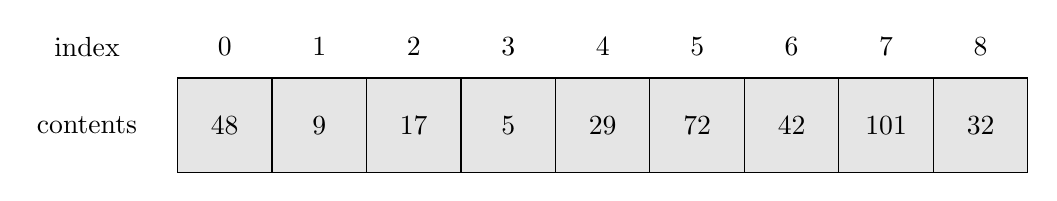
\begin{tikzpicture}
% size of each node
\def\sz{12mm}
% node style definition
\tikzstyle{block} = [
	draw, fill=black!10, rectangle,
	minimum height=\sz, minimum width=\sz ];
\tikzstyle{plain} = [draw=none,fill=none];
% array element definition
\node[plain] at (-1.75, 1) { index };
\node[plain] at (-1.75, 0) { contents };

\node[block] at (0*\sz,0) { 48 };
\node[plain] at (0*\sz,1.0) { 0 };
\node[block] at (1*\sz,0) { 9 };
\node[plain] at (1*\sz,1.0) { 1 };
\node[block] at (2*\sz,0) { 17 };
\node[plain] at (2*\sz,1.0) { 2 };
\node[block] at (3*\sz,0) { 5 };
\node[plain] at (3*\sz,1.0) { 3 };
\node[block] at (4*\sz,0) { 29 };
\node[plain] at (4*\sz,1.0) { 4 };
\node[block] at (5*\sz,0) { 72 };
\node[plain] at (5*\sz,1.0) { 5 };
\node[block] at (6*\sz,0) { 42 };
\node[plain] at (6*\sz,1.0) { 6 };
\node[block] at (7*\sz,0) { 101 };
\node[plain] at (7*\sz,1.0) { 7 };
\node[block] at (8*\sz,0) { 32 };
\node[plain] at (8*\sz,1.0) { 8 };

\end{tikzpicture}
\end{center}

\end{frame}


\begin{frame}[fragile]
    \frametitle{Indexing}
    \framesubtitle{}

\begin{itemize}[<+->]
  \item Suppose \mintinline{c}{arr} is an integer (4 bytes each) array
  \item \mintinline{c}{arr} is actually a \emph{memory address} 
  \item $i$-th element is at \mintinline{c}{arr[i]}
  \item Indexing automatically computes a \emph{memory offset}
  \item $i$-the element is 
   $$i \times 4$$
   bytes away from the beginning of the array
\end{itemize}

\end{frame}

\begin{frame}[fragile]
    \frametitle{Memory Offsets}
    \framesubtitle{}
    
\begin{center}    
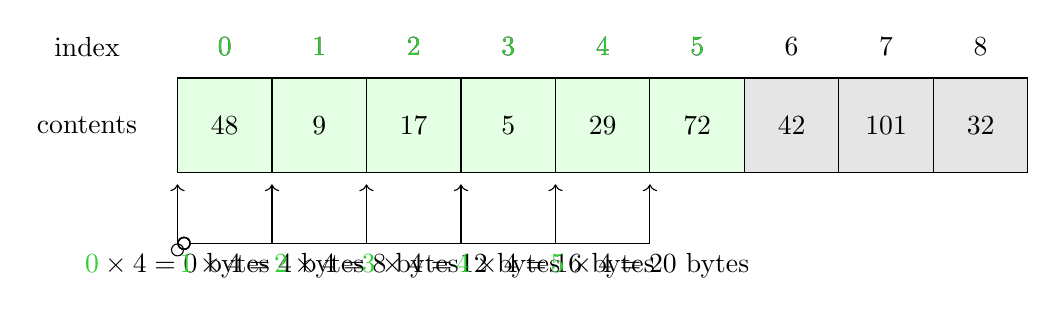
\begin{tikzpicture}
% size of each node
\def\sz{12mm}
% node style definition
\tikzstyle{block} = [
	draw, fill=black!10, rectangle,
	minimum height=\sz, minimum width=\sz ];
\tikzstyle{plain} = [draw=none,fill=none];
% array element definition
\node[plain] at (-1.75, 1) { index };
\node[plain] at (-1.75, 0) { contents };

\node[block] at (0*\sz,0) { 48 };
\node[plain] at (0*\sz,1.0) { 0 };
\node[block] at (1*\sz,0) { 9 };
\node[plain] at (1*\sz,1.0) { 1 };
\node[block] at (2*\sz,0) { 17 };
\node[plain] at (2*\sz,1.0) { 2 };
\node[block] at (3*\sz,0) { 5 };
\node[plain] at (3*\sz,1.0) { 3 };
\node[block] at (4*\sz,0) { 29 };
\node[plain] at (4*\sz,1.0) { 4 };
\node[block] at (5*\sz,0) { 72 };
\node[plain] at (5*\sz,1.0) { 5 };
\node[block] at (6*\sz,0) { 42 };
\node[plain] at (6*\sz,1.0) { 6 };
\node[block] at (7*\sz,0) { 101 };
\node[plain] at (7*\sz,1.0) { 7 };
\node[block] at (8*\sz,0) { 32 };
\node[plain] at (8*\sz,1.0) { 8 };

\onslide<2>{
\draw[black,o->] (-6mm, -1.5) -- (0*\sz-6mm, -1.5) -| node[below] {${\color{limegreen}{0}} \times 4 = 0$ bytes} (0*\sz-6mm, -0.75);
\node[block,fill=green!10] at (0*\sz,0) { 48 };
\node[plain] at (0*\sz,1.0) { \color{limegreen}{0} };
}
\onslide<3>{
\draw[black,o->] (-6mm, -1.5) -- (1*\sz-6mm, -1.5) -| node[below] {${\color{limegreen}{1}} \times 4 = 4$ bytes} (1*\sz-6mm, -0.75);
\node[block,fill=green!10] at (1*\sz,0) { 9 };
\node[plain] at (1*\sz,1.0) { \color{limegreen}{1} };
}
\onslide<4>{
\draw[black,o->] (-6mm, -1.5) -- (2*\sz-6mm, -1.5) -| node[below] {${\color{limegreen}{2}} \times 4 = 8$ bytes} (2*\sz-6mm, -0.75);
\node[block,fill=green!10] at (2*\sz,0) { 17 };
\node[plain] at (2*\sz,1.0) { \color{limegreen}{2} };
}
\onslide<5>{
  \draw[black,o->] (-6mm, -1.5) -- (3*\sz-6mm, -1.5) -| node[below] {${\color{limegreen}{3}} \times 4 = 12$ bytes} (3*\sz-6mm, -0.75);
  \node[block,fill=green!10] at (3*\sz,0) { 5 };
\node[plain] at (3*\sz,1.0) { \color{limegreen}{3} };
}
\onslide<6>{
  \draw[black,o->] (-6mm, -1.5) -- (4*\sz-6mm, -1.5) -| node[below] {${\color{limegreen}{4}} \times 4 = 16$ bytes} (4*\sz-6mm, -0.75);
  \node[block,fill=green!10] at (4*\sz,0) { 29 };
  \node[plain] at (4*\sz,1.0) { \color{limegreen}{4} };
}
\onslide<7>{
  \draw[black,o->] (-6mm, -1.5) -- (5*\sz-6mm, -1.5) -| node[below] {${\color{limegreen}{5}} \times 4 = 20$ bytes} (5*\sz-6mm, -0.75);
  \node[block,fill=green!10] at (5*\sz,0) { 72 };
  \node[plain] at (5*\sz,1.0) { \color{limegreen}{5} };
}
\end{tikzpicture}
\end{center}

\end{frame}

\section{Using Arrays}

\begin{frame}
    \frametitle{}
    \framesubtitle{}
    
    \begin{center}
    {\Huge Part II: Using Arrays}\\
    {\Large ~}
    \end{center}

\end{frame}


\begin{frame}[fragile]
    \frametitle{Using Arrays}
    \framesubtitle{}

\begin{itemize}[<+->]
  \item Static arrays are allocated on the program stack
  \item Declaration specifies size
  \item[~]
\begin{minted}{c}
int arr[10];
double numbers[20];
\end{minted}
  \item Once declared, indexing can be used to access values
\begin{minted}{c}
arr[0] = 42;
arr[1] = 12;
arr[2] = arr[0] + 20;
arr[9] = 3.75; //truncation

printf("a[0] = %d\n", a[0]); 
\end{minted}
\end{itemize}

\end{frame}

\begin{frame}[fragile]
    \frametitle{Alternative Syntax}
    \framesubtitle{Declaration/initialization}

\begin{itemize}[<+->]
  \item You can declare and initialize an array at the same time
  \item[~]
\begin{minted}{c}
int primes[] = { 2, 3, 5, 7, 11, 13, 17 };
\end{minted}
  \item Size specification is \emph{optional}
  \item Example of \emph{code elision} 
  \item Problem: You still need to keep track of the \emph{size} of the array
\end{itemize}

\end{frame}


\begin{frame}[fragile]
    \frametitle{Variable Length Arrays}
    \framesubtitle{}

\begin{itemize}[<+->]
  \item C99+ allows you to declare an array with a variable size
  \item[~]
\begin{minted}{c}
int n = 10;
int arr[n];
\end{minted}
  \item Just because you \emph{can} (or more accurately \emph{might}) 
    be able to do this, doesn't mean you should
  \item Avoid in general
\end{itemize}

\end{frame}

\begin{frame}[fragile]
    \frametitle{Pitfalls}
    \framesubtitle{Uninitialized Arrays}

\begin{itemize}[<+->]
  \item Like regular variables, there is \emph{no default value}
  \item \mintinline{c}{arr[3]} was not set, its value could be anything
  \item Never make assumptions about uninitialized variables
  \item Always initialize yourself
\end{itemize}

\end{frame}

\begin{frame}[fragile]
    \frametitle{Pitfalls}
    \framesubtitle{Out-of-bounds indexing}

\begin{itemize}[<+->]  
  \item Accessing invalid indices is \emph{undefined behavior}
  \item[~]
\begin{minted}{c}
int arr[10];
...
arr[10] = 42;
arr[-1] = 21;
\end{minted}
  \item May lead to:
  \begin{itemize}
    \item A segmentation fault, bus error
    \item Corrupted memory
    \item Incorrect results
  \end{itemize}
  \item \emph{Your} responsibility to do \emph{bookkeeping}
\end{itemize}

\end{frame}

\begin{frame}[fragile]
    \frametitle{Pitfalls}
    \framesubtitle{Book Keeping}

\begin{itemize}[<+->]  
  \item You must always keep track of the size of an array
  \item In general there is no way to determine the size of an array
  \item Only in very limited situations (static arrays)
  \item Arrays should be accompanied by an integer variable to keep 
  track of its size
  \item Idiomatic loops over arrays
  \item Demonstration
\end{itemize}
\end{frame}

\begin{frame}[fragile]
    \frametitle{Pitfalls}
    \framesubtitle{Book Keeping}
    
\begin{minted}{c}
int n = 10;
int primes[] = { 2, 3, 5, 7, 11, 13, 17, 19, 23, 29 };
int sum = 0;

for(int i=0; i<n; i++) {
  sum += primes[i];
}
\end{minted}

\end{frame}

\section{Dynamic Arrays}

\begin{frame}
    \frametitle{}
    \framesubtitle{}
    
    \begin{center}
    {\Huge Part III: Dynamic Arrays}\\
    {\Large ~}
    \end{center}

\end{frame}

\begin{frame}[fragile]
    \frametitle{Static Arrays are Insufficient}
    \framesubtitle{}

\begin{itemize}[<+->]  
  \item Static arrays are allocated on the program stack
  \item Inside a stack frame in which it is declared
  \item Stack space is \emph{limited} 
  \item 8MB (large) to 64k or even 8k (embedded systems)
  %demo: ulimit -a
  \item Demonstration  
  %\item In any 
  %TODO: don't abuse the stack space
  %example with VLA and with hard-coded value
\end{itemize}

\end{frame}

\begin{frame}[fragile]
    \frametitle{Static Arrays are Insufficient}
    \framesubtitle{}

\begin{itemize}[<+->]  
  \item Stack is small, inappropriate to hold even ``moderately' sized arrays
  \item Other disadvantages: static arrays cannot be returned from functions
  \item Best to not use static arrays at all
  \item Don't abuse the stack space, it is small and defenseless 
  \item Better solution: use \emph{dynamic arrays}
\end{itemize}

\end{frame}

\begin{frame}[fragile]
    \frametitle{Dynamic Memory \& Arrays}
    \framesubtitle{}

\begin{itemize}[<+->]  
  \item Dynamic memory is allocated in a program's \emph{heap}
  \item Stack: highly organized, efficient, but small/limited
  \item Heap: Less organized, less efficient, but much larger
  \item Dynamically allocate memory on the heap using 
  \mintinline{c}{malloc()} (\textbf{M}emory \textbf{Alloc}ation)
\end{itemize}
\end{frame}

\begin{frame}[fragile]
    \frametitle{malloc}
    \framesubtitle{}

\begin{itemize}[<+->]  
  \item Located in the standard library \mintinline{c}{stdlib.h}
  \item Takes one argument: the number of bytes you want to allocate
  \item Use \mintinline{c}{sizeof()} to determine how many bytes each type of variable takes
  \item Returns a generic \emph{void pointer}: \mintinline{c}{void *}
  \item A void pointer points to a generic memory location that can be 
  \emph{cast} to any type you want
  \item Returns \mintinline{c}{NULL} if unsuccessful
  \item Demonstration
  %from the failed demonstration, update it to use malloc, several steps:
  % add type cast
  % hard-code size, then modify to use sizeof
  % add error checking
  % add another example using doubles
\end{itemize}

\end{frame}



\section{Memory Management}

\begin{frame}
    \frametitle{}
    \framesubtitle{}
    
    \begin{center}
    {\Huge Part IV: Memory Management}\\
    {\Large ~}
    \end{center}

\end{frame}

\begin{frame}[fragile]
    \frametitle{Overview}
    \framesubtitle{}

\begin{itemize}[<+->]  
  \item Memory on the stack is ``cleaned up'' when stack frames are removed
  \item Memory on the heap is \emph{not} automatically cleaned up when it is no longer needed
  \item It is \emph{your} responsibility to ``clean up'' dynamically allocated memory when you no longer need it
  \item Failure to do so or failure to do so correctly can lead to:
  \begin{itemize}
    \item Memory Leaks
    \item Reduced performance
    \item Illegal memory access/segmentation faults
  \end{itemize}
\end{itemize}

\end{frame}

\begin{frame}[fragile]
    \frametitle{Freeing Memory}
    \framesubtitle{}

\begin{itemize}[<+->]  
  \item To clean up memory you ``free'' it
  \item Standard library function: \\
    \mintinline{c}{void free(void *)}
  \item Takes a single argument: a pointer to dynamically allocated memory
  \item Demonstration
\end{itemize}

\end{frame}

\begin{frame}[fragile]
    \frametitle{Demonstration}
    \framesubtitle{}

\begin{minted}{c}
#include<stdlib.h>
#include<stdio.h>
int main(int argc, char **argv) {

  int n = 100;
  int *arr = (int *) malloc(n * sizeof(int));

  //process the array
  for(int i=0; i<n; i++) {
    arr[i] = (i+1);
  }

  free(arr);

  return 0;
}
\end{minted}

\end{frame}

\begin{frame}[fragile]
    \frametitle{Pitfall}
    \framesubtitle{Dangling Pointers}

\begin{itemize}[<+->]  
  \item Basic usage is easy, though there are many pitfalls
  \item Once freed, dynamic memory cannot/should not be accessed
  \item Best to \emph{reset} the pointer to \mintinline{c}{NULL}
  \item Otherwise, it is a \emph{dangling pointer}
  \item Demonstration
\end{itemize}

\end{frame}

\begin{frame}[fragile]
    \frametitle{Pitfall}
    \framesubtitle{Dangling Pointers}

\begin{minted}{c}
int *arr = (int *) malloc(n * sizeof(int));
//...
free(arr);

//arr still points to a memory location, but is no longer valid
printf("arr points to %p\n", arr);
//accessing is undefined behavior:
arr[0] = 42;

//best to reset to NULL;
free(arr);
arr = NULL;
\end{minted}

\end{frame}

\begin{frame}[fragile]
    \frametitle{Pitfall}
    \framesubtitle{Memory Ownership}

\begin{itemize}[<+->]  
  \item Different sections of code may ``own'' memory and be responsible for its management
  \item Stack frames are ``owned'' by the program/function: the program is responsible for clean up 
  \item Ownership may be transferred: \mintinline{c}{malloc} transfers ownership to the calling function
  \item Ownership is a design issue/decision
  \item In general: only \mintinline{c}{free} memory if you own it
  \item Don't \mintinline{c}{free} memory before you are done with it
  \item Don't \mintinline{c}{free} freed memory
\end{itemize}

\end{frame}

\begin{frame}[fragile]
    \frametitle{Pitfall}
    \framesubtitle{Memory Leaks}

\begin{itemize}[<+->]  
  \item Failure to properly clean up memory can lead to \emph{memory leaks}
  \item A program holds on to memory it doesn't use
  \item Or: references are lost to memory that cannot be freed
  \item Program takes more and more resources 
  \item Performance degrades, taking the entire system down with it
  \item Demonstration
  %must do it on CSE; mac doesn't show virtual memory?  
\end{itemize}
  
\end{frame}

\section{Arrays \& Functions}

\begin{frame}
    \frametitle{}
    \framesubtitle{}
    
    \begin{center}
    {\Huge Part V: Arrays \& Functions}\\
    {\Large ~}
    \end{center}

\end{frame}

\begin{frame}[fragile]
    \frametitle{Using Arrays With Functions}
    \framesubtitle{~}

\begin{itemize}[<+->]  
  \item Goal: use arrays with functions
  \item Pass arrays to functions
  \item Return arrays from functions
  \item Recall: you always need to do your own \emph{bookkeeping} with arrays
  \item Anytime you pass an array, you also need to pass its \emph{size}
  \item Anytime you return an array, you need a way to implicitly determine its size
\end{itemize}

\end{frame}

\begin{frame}[fragile]
    \frametitle{Demonstration}
    \framesubtitle{~}

Write a function that takes an array of integers and returns the
sum of its values.

\end{frame}

\begin{frame}[fragile]
    \frametitle{Demonstration}
    \framesubtitle{~}

\begin{minted}{c}    
/**
 * This function takes an integer array (of size n) and
 * returns the sum of its elements.  It returns 0 if the
 * array is NULL.
 */
int sum(int *arr, int n) {

  if(arr == NULL) {
    return 0;
  }
  int total = 0;
  for(int i=0; i<n; i++) {
    total += arr[i];
  }
  return total;
}
\end{minted}
\begin{itemize}
  \item Since arrays are passed by reference, no ampersands are needed.
  \item Technically using the square brackets automatically dereferences the elements in the array (the square bracket syntax means we don't have to do our own pointer arithmetic)
\end{itemize}

\end{frame}

\begin{frame}[fragile]
    \frametitle{The \texttt{const} Keyword}
    \framesubtitle{~}
    

\begin{itemize}[<+->]
  \item Arrays are \emph{always} passed by reference in C
  \item It is possible to make changes to their contents
  \item We don't always want this
  \item We can add the keyword \mintinline{c}{const} to prevent changes to the array
  \item The compiler checks for changes and generates an error if this ``promise'' is violated
  \item Design issue, not a full guarantee
  \item Demonstration
  %show that changes can be made by settting them to zero before adding
  %add const to prevent this
\end{itemize}
  
\end{frame}

\begin{frame}[fragile]
    \frametitle{Returning Arrays}
    \framesubtitle{~}
    
\begin{itemize}[<+->]  
  \item Functions can create and return arrays
  \item You \emph{cannot} return static arrays
  \item Only dynamic arrays can be returned
  \item Demonstration
\end{itemize}
  
\end{frame}

\begin{frame}[fragile]
    \frametitle{Returning Arrays}
    \framesubtitle{~}
    
\begin{minted}{c}
#include <stdlib.h> 
#include <stdio.h>

int * foo() {
  int b[3];
  b[0] = 10;
  b[1] = 20;
  b[2] = 30;
  return b; 
}

int main(int argc, char **argv) {
  int *a = foo();
  for(int i=0; i<3; i++) {
    printf("a[%d] = %d\n", i, a[i]);
  }
  return 0; 
}
\end{minted}  

\end{frame}

\begin{frame}[fragile]
    \frametitle{Exercises}
    \framesubtitle{~}

\begin{itemize}
  \item Write a function that takes an integer $n$ and returns
  an array of $n$ integers, all initialized to 1
%  \item Write a function to compute the average of elements in
%  an integer array
  \item Write a function that takes an integer array and returns a new
  \emph{copy} of the array with all instances of zero removed 
\end{itemize}
  
\end{frame}

\section{Multi-dimensional Arrays}

\begin{frame}
    \frametitle{}
    \framesubtitle{}
    
    \begin{center}
    {\Huge Part VI: Multidimensional Arrays}\\
    {\Large ~}
    \end{center}

\end{frame}

\begin{frame}[fragile]
    \frametitle{Multidimensional Arrays}
    \framesubtitle{~}

\begin{itemize}[<+->]  
  \item Up to now: 1-dimensional arrays
  \item You can have arrays with more than one dimension
  \item 2-D arrays: 
  \begin{itemize}
    \item Rows \& columns
    \item Tabular data
    \item Matrices
  \end{itemize}
  \item 3-D arrays:
  \begin{itemize}
    \item Rows, columns, \& ``lanes'' 
    \item 3-dimensional data
  \end{itemize}
  \item 4+ dimensional arrays:
  \begin{itemize}
    \item Rethink what you're doing
  \end{itemize}
  \item Focus on 2-D arrays
\end{itemize}

\end{frame}

\begin{frame}[fragile]
    \frametitle{Multidimensional Arrays}
    \framesubtitle{~}

\begin{itemize}[<+->]  
  \item A pointer, \mintinline{c}{int *arr} points to a 1-dimensional array
  \item A ``double'' pointer, \mintinline{c}{int **mat} points to a ``2-dimensional array''
  \item Technically points to an array of pointers
  \item Each pointer in the array points to an array of integers
  \item Demonstration
\end{itemize}

\end{frame}

\begin{frame}[fragile]
    \frametitle{Multidimensional Arrays}
    \framesubtitle{~}

\begin{minted}{c}
int n = 10;
int **matrix = NULL;
matrix = (int **) malloc(n * sizeof(int*));
for(int i=0; i<n; i++) {
  matrix[i] = (int *) malloc(n * sizeof(int));
}
\end{minted}  

\end{frame}

\begin{frame}[fragile]
    \frametitle{Multidimensional Arrays}
    \framesubtitle{~}

\begin{tikzpicture}[scale=.75,transform shape]

% Define block styles
\tikzstyle{box} = [rectangle,
                   fill=white,
                   %draw,
                   text width=2.5cm,
                   text centered,
%                   rounded corners,
%                   minimum height=4em,
                   inner sep=2.5pt,
                   node distance=.60cm]

\tikzstyle{line} = [draw, -latex']; 

  \node [text width = 15cm] at (7,2) {
\begin{minted}{c}
int n = 10;
int **matrix = NULL; 
matrix = (int **) malloc(n * sizeof(int*)); 
for(int i=0; i<n; i++) {
  matrix[i] = (int *) malloc(n * sizeof(int));
}
\end{minted}
 };

    \node [box] (init) at (0,0) {\mintinline{c}{**matrix}};
\onslide<2->
{
    \node [box, below of=init,node distance=1cm] (p0) {\mintinline{c}{*matrix[0]}};
    \node [box, below of=p0] (p1) {\mintinline{c}{*matrix[1]}};
    \node [box, below of=p1] (p2) {\mintinline{c}{*matrix[2]}};
    \node [below of=p2,node distance=1cm] (pd) {$\vdots$};
    \node [box, below of=pd,node distance=1cm] (pn) {\mintinline{c}{*matrix[n-1]}};
    \path [line] (init) -- (p0);
}

\onslide<3->{
    \node [box, right of=p0,node distance=4cm] (m00) {\mintinline{c}{matrix[0][0]}};
    \node [box, right of=m00,node distance=3cm] (m01) {\mintinline{c}{matrix[0][1]}};
    \node [box, right of=m01,node distance=3cm] (m02) {\mintinline{c}{matrix[0][2]}};
    \node [right of=m02,node distance=2.25cm] (m0d) {$\cdots$};
    \node [box, text width=3.2cm, right of=m0d,node distance=2.5cm] (m0n) {\mintinline{c}{matrix[0][n-1]}};
    \path [line] (p0) -- (m00);
}
\onslide<4->{
    \node [box, right of=p1,node distance=4cm] (m10) {\mintinline{c}{matrix[1][0]}};
    \node [box, right of=m10,node distance=3cm] (m11) {\mintinline{c}{matrix[1][1]}};
    \node [box, right of=m11,node distance=3cm] (m12) {\mintinline{c}{matrix[1][2]}};
    \node [right of=m12,node distance=2.25cm] (m1d) {$\cdots$};
    \node [box, text width=3.2cm, right of=m1d,node distance=2.5cm] (m1n) {\mintinline{c}{matrix[1][n-1]}};
    \path [line] (p1) -- (m10);
}
\onslide<5->{
    \node [box, right of=p2,node distance=4cm]    (m20) {\mintinline{c}{matrix[2][0]}};
    \node [box, right of=m20,node distance=3cm] (m21) {\mintinline{c}{matrix[2][1]}};
    \node [box, right of=m21,node distance=3cm] (m22) {\mintinline{c}{matrix[2][2]}};
    \node [right of=m22,node distance=2.25cm]        (m2d) {$\cdots$};
    \node [box, text width=3.2cm, right of=m2d,node distance=2.5cm]   (m2n) {\mintinline{c}{matrix[2][n-1]}};
    \path [line] (p2) -- (m20);
}
\onslide<6->{
    \node [box, right of=pn,node distance=4cm]    (mn0) {\mintinline{c}{matrix[n-1][0]}};
    \node [box, right of=mn0,node distance=3cm] (mn1) {\mintinline{c}{matrix[n-1][1]}};
    \node [box, right of=mn1,node distance=3cm] (mn2) {\mintinline{c}{matrix[n-1][2]}};
    \node [right of=mn2,node distance=2.25cm]        (mnd) {$\cdots$};
    \node [box, text width=3.6cm, right of=mnd,node distance=2.5cm]   (mnn) {\mintinline{c}{matrix[n-1][n-1]}};
    \path [line] (pn) -- (mn0);
}

\end{tikzpicture}

\end{frame}

\begin{frame}[fragile]
    \frametitle{Usage}
    \framesubtitle{~}

\begin{itemize}[<+->]  
  \item Once created, you can access elements using \emph{two} indices
  \item Usually: row-column interpretation
  \item \mintinline{c}{matrix[i][j]} accesses the $i$-th row and $j$-th column
  \item Use two nested for-loops to iterate over each row/column
  \item[~]
\begin{minted}{c}
for(int i=0; i<n; i++) {
  for(int j=0; j<n; j++) {
    matrix[i][j] = (2*i+3*j);
  }
}
printf("last row/column value = %d\n", matrix[n-1][n-1]);
\end{minted}
\end{itemize}

\end{frame}

\begin{frame}[fragile]
    \frametitle{Demo}
    \framesubtitle{~}
    

\begin{minted}{c}
#include<stdlib.h>
#include<stdio.h>

int main(int argc, char **argv) {

  int n = 3;
  int **matrix = NULL;
  matrix = (int **) malloc(n * sizeof(int*));
  for(int i=0; i<n; i++) {
    matrix[i] = (int *) malloc(n * sizeof(int));
  }

  int value = 1;
  for(int i=0; i<n; i++) {
    for(int j=0; j<n; j++) {
      matrix[i][j] = value;
      value++;
    }
  }

  return 0;
}
\end{minted}
\end{frame}

\begin{frame}[fragile]
    \frametitle{Clean Up}
    \framesubtitle{~}

\begin{itemize}[<+->]  
  \item Must do proper cleanup when freeing 2-D arrays
  \item Cannot simply free the matrix:
  \mintinline{c}{free(matrix)}
  \item Results in a memory leak
  \item You must free each row before you free the array of pointers
  \item[~]  
\begin{minted}{c}
for(int i=0; i<n; i++) {
  free(matrix[i]);
}
free(matrix);
\end{minted}
\end{itemize}
  
\end{frame}

\begin{frame}[fragile]
    \frametitle{Alternative: Contiguous Allocation}
    \framesubtitle{~}

\begin{minted}{c}
#include<stdlib.h>

int main(int argc, char **argv) {

  int n = 5, m = 3;
  int **arr = (int **)malloc(sizeof(int *) * n);
  arr[0] = (int *)malloc(sizeof(int) * (n * m));

  for(int i=1; i<n; i++) {
    arr[i] = (*arr + (m * i));
  }
  
  int value = 1;
  for(int i=0; i<n; i++) {
    for(int j=0; j<m; j++) {
      arr[i][j] = value;
      value++;
    }
  }
  return 0;
}
\end{minted}
\end{frame}

\section{Shallow vs Deep}

\begin{frame}
    \frametitle{}
    \framesubtitle{}
    
    \begin{center}
    {\Huge Part VII: Shallow vs.\ Deep Copies}\\
    {\Large ~}
    \end{center}

\end{frame}


\begin{frame}[fragile]
    \frametitle{Shallow Copy}
    \framesubtitle{}

Consider the following piece of code, what does it print?
\begin{minted}{c}
//create an array containing {10, 20, 30, 40, 50}
int n = 5;
int *a = (int *) malloc(n * sizeof(int));
for(int i=0; i<n; i++) {
  a[i] = (i+1)*10;
}

//let's make a "copy"
int *b = a;
b[0] = 42;

//what is in a[0]?
printf("a[0] = %d\n", a[0]);
\end{minted}

%DEMO

\end{frame}


\begin{frame}[fragile]
    \frametitle{Shallow Copy}
    \framesubtitle{}


\begin{center}
\begin{tikzpicture}
% size of each node
\def\sz{10mm}
% node style definition
\tikzstyle{block} = [
	draw, fill=black!10, rectangle,
	minimum height=\sz, minimum width=\sz ];
\tikzstyle{plain} = [draw=none,fill=none];

\node[plain] (a) at (-2, 0) { \mintinline{c}{a} };

\node[block] (c) at (0,0) { ~ };

\draw[->] (a) -- (c);

\node[block] at (0*\sz,0) { 10 };
\node[plain] at (0*\sz,1.0) { 0 };
\node[block] at (1*\sz,0) { 20 };
\node[plain] at (1*\sz,1.0) { 1 };
\node[block] at (2*\sz,0) { 30 };
\node[plain] at (2*\sz,1.0) { 2 };
\node[block] at (3*\sz,0) { 40 };
\node[plain] at (3*\sz,1.0) { 3 };
\node[block] at (4*\sz,0) { 50 };
\node[plain] at (4*\sz,1.0) { 4 };


\onslide<2->{
  \node[plain] (b) at (-2, -2) { \mintinline{c}{b} };
  \draw[->] (b) -- (a);
}
\onslide<2-3>{
  \node at (2,-2) {\mintinline{c}{int *b = a;}};
}
\onslide<3->{
  \draw[->,dashed,shorten >=.1cm] (b.north) to [bend left] (c.west);
}
\onslide<4->{
  \node[draw, fill=red!30, rectangle,
	    minimum height=\sz, minimum width=\sz] at (0*\sz,0) { 42 };
}
\onslide<4>{
  \node at (2,-2) {\mintinline{c}{b[0] = 42;}};
}

\end{tikzpicture}
\end{center}
\end{frame}

\begin{frame}[fragile]
    \frametitle{Shallow Copy}
    \framesubtitle{}

\begin{itemize}[<+->]
  \item A shared reference is a \emph{shallow copy}
  \item Multiple pointers refer to the same memory location/array
  \item Changes to one reference affect the other
  \item Not typically what we want with a ``copy''
\end{itemize}

\end{frame}

\begin{frame}[fragile]
    \frametitle{Deep Copy}
    \framesubtitle{}

\begin{itemize}[<+->]
  \item In contrast: a \emph{deep copy} is when we have two 
  \emph{separate} arrays with the same \emph{contents}
  \item Two \emph{different} memory locations
  \item Changes to one do not affect the other
  \item Example
  \item Demo: write a deep copy function
\end{itemize}

\end{frame}


\begin{frame}[fragile]
    \frametitle{Deep Copy}
    \framesubtitle{}


\begin{center}
\begin{tikzpicture}
% size of each node
\def\sz{10mm}
% node style definition
\tikzstyle{block} = [
	draw, fill=black!10, rectangle,
	minimum height=\sz, minimum width=\sz ];
\tikzstyle{plain} = [draw=none,fill=none];

\node[plain] (a) at (-2, 0) { \mintinline{c}{a} };
\node[block] (c) at (0,0) { ~ };
\draw[->] (a) -- (c);
\node[block] at (0*\sz,0) { 10 };
\node[plain] at (0*\sz,1.0) { 0 };
\node[block] at (1*\sz,0) { 20 };
\node[plain] at (1*\sz,1.0) { 1 };
\node[block] at (2*\sz,0) { 30 };
\node[plain] at (2*\sz,1.0) { 2 };
\node[block] at (3*\sz,0) { 40 };
\node[plain] at (3*\sz,1.0) { 3 };
\node[block] at (4*\sz,0) { 50 };
\node[plain] at (4*\sz,1.0) { 4 };

\node[plain] (b) at (-2, -3) { \mintinline{c}{b} };
\node[block] (d) at (0,-3) { ~ };
\draw[->] (b) -- (d);
\node[block] at (0*\sz,-3) { 10 };
\node[plain] at (0*\sz,-2) { 0 };
\node[block] at (1*\sz,-3) { 20 };
\node[plain] at (1*\sz,-2) { 1 };
\node[block] at (2*\sz,-3) { 30 };
\node[plain] at (2*\sz,-2) { 2 };
\node[block] at (3*\sz,-3) { 40 };
\node[plain] at (3*\sz,-2) { 3 };
\node[block] at (4*\sz,-3) { 50 };
\node[plain] at (4*\sz,-2) { 4 };

\onslide<2>{
  \node[draw, fill=red!30, rectangle,
	    minimum height=\sz, minimum width=\sz] at (0*\sz,-3) { 42 };
  \node at (1,-5) {\mintinline{c}{b[0] = 42;}};
}

\end{tikzpicture}
\end{center}
\end{frame}


\begin{frame}[fragile]
    \frametitle{Deep Copy}
    \framesubtitle{}

\begin{minted}{c}
/**
 * This function creates a deep copy of the
 * given array.
 */
int * deepCopy(const int *a, int n) {
  if(a == NULL || n < 0) {
    return NULL;
  }
  int *copy = (int *) malloc(n * sizeof(int));
  for(int i=0; i<n; i++) {
    copy[i] = a[i];
  }
  return copy;
}
\end{minted}
\end{frame}

\end{document} 
